\graphicspath{{/home/maurizio/Documents/GitHub/computational-biophysics-theory/pathria/images/}}

\section{Cartesian to polar coordinates mometnum}

Certainly! Let's derive the differential volume element in momentum space, \(d^3p\), using spherical coordinates step by step.

Step 1: Cartesian to Spherical Coordinates
In Cartesian coordinates, the momentum vector \(\vec{p}\) is given by components \(p_x\), \(p_y\), and \(p_z\). In spherical coordinates, this same vector is represented by \(p\), \(\theta\), and \(\phi\), where:
- \( p \) is the magnitude of the momentum vector.
- \(\theta\) is the polar angle, measured from the \(z\)-axis.
- \(\phi\) is the azimuthal angle, measured in the \(xy\)-plane from the \(x\)-axis.

The relationships between Cartesian and spherical coordinates are:
- \( p_x = p \sin\theta \cos\phi \)
- \( p_y = p \sin\theta \sin\phi \)
- \( p_z = p \cos\theta \)

Step 2: Differential Volume Element in Cartesian Coordinates
In Cartesian coordinates, the differential volume element is:
\[ d^3p = dp_x \, dp_y \, dp_z \]

Step 3: Transforming the Differential Volume Element
We need to transform \(dp_x \, dp_y \, dp_z\) into spherical coordinates \(p, \theta, \phi\). This transformation requires the Jacobian determinant of the transformation from \((p_x, p_y, p_z)\) to \((p, \theta, \phi)\).

The Jacobian matrix \(J\) for the transformation is:
\[ J = \begin{pmatrix}
\frac{\partial p_x}{\partial p} & \frac{\partial p_x}{\partial \theta} & \frac{\partial p_x}{\partial \phi} \\
\frac{\partial p_y}{\partial p} & \frac{\partial p_y}{\partial \theta} & \frac{\partial p_y}{\partial \phi} \\
\frac{\partial p_z}{\partial p} & \frac{\partial p_z}{\partial \theta} & \frac{\partial p_z}{\partial \phi}
\end{pmatrix} \]

Calculating the partial derivatives:
\[ \frac{\partial p_x}{\partial p} = \sin\theta \cos\phi \]
\[ \frac{\partial p_x}{\partial \theta} = p \cos\theta \cos\phi \]
\[ \frac{\partial p_x}{\partial \phi} = -p \sin\theta \sin\phi \]

\[ \frac{\partial p_y}{\partial p} = \sin\theta \sin\phi \]
\[ \frac{\partial p_y}{\partial \theta} = p \cos\theta \sin\phi \]
\[ \frac{\partial p_y}{\partial \phi} = p \sin\theta \cos\phi \]

\[ \frac{\partial p_z}{\partial p} = \cos\theta \]
\[ \frac{\partial p_z}{\partial \theta} = -p \sin\theta \]
\[ \frac{\partial p_z}{\partial \phi} = 0 \]

Thus, the Jacobian matrix \(J\) is:
\[ J = \begin{pmatrix}
\sin\theta \cos\phi & p \cos\theta \cos\phi & -p \sin\theta \sin\phi \\
\sin\theta \sin\phi & p \cos\theta \sin\phi & p \sin\theta \cos\phi \\
\cos\theta & -p \sin\theta & 0
\end{pmatrix} \]

Step 4: Determinant of the Jacobian Matrix
The volume element \(d^3p\) in spherical coordinates is given by the absolute value of the determinant of \(J\):
\[ \left| \det(J) \right| dp \, d\theta \, d\phi \]

Calculating the determinant of \(J\):
\begin{align*}
    \frac{\partial (x, y, z)}{\partial (p, \theta, \phi)} &=
    \begin{vmatrix}
    \sin\theta \cos\phi & p \cos\theta \cos\phi & -p \sin\theta \sin\phi \\
    \sin\theta \sin\phi & p \cos\theta \sin\phi & p \sin\theta \cos\phi \\
    \cos\theta & -p \sin\theta & 0
    \end{vmatrix} \\
    &= \sin\theta \cos\phi \left( p \cos\theta \sin\phi \cdot 0 - p \sin\theta \cos\phi \cdot (-p \sin\theta) \right) \\
    &\quad - p \cos\theta \cos\phi \left( \sin\theta \sin\phi \cdot 0 - p \sin\theta \cos\phi \cdot \cos\theta \right) \\
    &\quad - p \sin\theta \sin\phi \left( \sin\theta \sin\phi \cdot (-p \sin\theta) - p \cos\theta \sin\phi \cdot \cos\theta \right) \\
    &= \sin\theta \cos\phi \left( p^2 \sin^2\theta \cos\phi \right) \\
    &\quad - p \cos\theta \cos\phi \left( -p \sin\theta \cos\theta \cos\phi \right) \\
    &\quad - p \sin\theta \sin\phi \left( -p \sin^2\theta \sin\phi - p \cos^2\theta \sin\phi \right) \\
    &= p^2 \sin^3\theta \cos^2\phi + p^2 \cos^2\theta \sin\theta \cos^2\phi + p^2 \sin\theta \left( \sin^2\theta + \cos^2\theta \right) \sin^2\phi \\
    &= p^2 \sin\theta \left( \sin^2\theta \cos^2\phi + \cos^2\theta \cos^2\phi + \sin^2\phi \right) \\
    &= p^2 \sin\theta \left( \cos^2\phi (\sin^2\theta + \cos^2\theta) + \sin^2\phi \right) \\
    &= p^2 \sin\theta \left( \cos^2\phi + \sin^2\phi \right) \\
    &= p^2 \sin\theta \cdot 1 \\
    &= p^2 \sin\theta.
    \end{align*}

Thus, the volume element in spherical coordinates is:
\[ d^3p = p^2 \sin\theta \, dp \, d\theta \, d\phi \]


Given this result, you can also derive the volume of a spherical shell using spherical coordinates.
To find the volume of a thin spherical shell of radius \(p\) and thickness \(dp\):

\begin{itemize}
    \item \textbf{Integration Over Angles}:
    Integrate over all angles \(\theta\) and \(\phi\):
    \[
    \text{Volume of shell} = \int_0^{2\pi} \int_0^\pi p^2 \sin \theta \, dp \, d\theta \, d\phi
    \]
    Here, \(dp\) is the thickness of the shell and is fixed in the shell volume computation.
 
    \item \textbf{Evaluate the Angular Integrals}:
    \[
    \int_0^{2\pi} d\phi = 2\pi
    \]
    \[
    \int_0^\pi \sin \theta \, d\theta = \left. -\cos \theta \right|_0^\pi = 2
    \]
 
    \item \textbf{Combine the Results}:
    \[
    \text{Volume of shell} = p^2 \left( \int_0^\pi \sin \theta \, d\theta \right) \left( \int_0^{2\pi} d\phi \right) \, dp
    \]
    \[
    \text{Volume of shell} = p^2 \cdot 2 \cdot 2\pi \cdot dp
    \]
    \[
    \text{Volume of shell} = 4\pi p^2 \, dp
    \]
 
\end{itemize}

So, indeed, using spherical coordinates and integrating over all angles confirms that the volume of a thin spherical shell of radius \(p\) and thickness \(dp\) is \(4 \pi p^2 \, dp\), aligning with the result obtained from the volume difference method.


\section{The Joule and Joule-Thomson Experiments}

\begin{figure}
    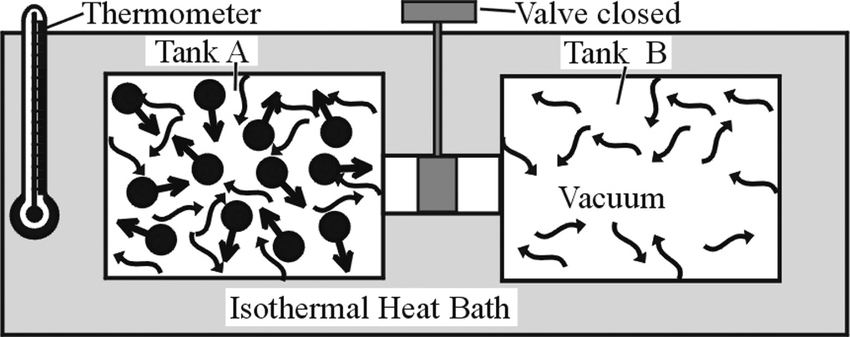
\includegraphics{/home/maurizio/Documents/GitHub/computational-biophysics-theory/pathria/images/joule_experiment.jpg}
    \caption{Joule experiment}
\end{figure}

Given that the change of energy in an adyabatic system can be written as

\begin{align*}
    dU &= \left(\frac{\partial U}{\partial V}\right)_T dV + \left(\frac{\partial U}{\partial T}\right)_V dT \\
       &= \left(\frac{\partial U}{\partial V}\right)_T dV + C_V dT
\end{align*}

Considering that

$$
d U = dQ + dW = C_P dT - PdV
$$

Than we have that 

\begin{align*}
    &C_P dT - PdV = \left(\frac{\partial U}{\partial V}\right)_T dV + C_V dT \\
    &C_P - P \left(\frac{dV}{dT}\right)_P = \left(\frac{\partial U}{\partial V}\right)_T \left(\frac{\partial V}{\partial T}\right)_P + C_V \\
    &C_P - C_V = \left[P + \left(\frac{\partial U}{\partial V}\right)_T\right] \left(\frac{\partial V}{\partial T}\right)_P
\end{align*}

It is possible to demonstrate that

$$
\left(\frac{\partial U}{\partial V}\right)_T = T \left(\frac{\partial P }{\partial T}\right)_V - P
$$

Therefore

\begin{equation}
    C_P - C_V = T \left(\frac{\partial P }{\partial T}\right)_V \left(\frac{\partial V }{\partial T}\right)_P
\end{equation}
